\section{Adopted Methodology}

In this section, we will discuss the methodology adopted for the development of our SaaS email marketing application.

\subsection{Methodology Choice}

For this project, we have chosen to adopt the SCRUM methodology \cite{scrum}. This decision was made due to several reasons. Firstly, SCRUM is an agile development methodology which allows for rapid iteration and flexibility. This is particularly important for our project as it allows us to quickly adapt to changes and continuously improve our product based on user feedback. Secondly, SCRUM promotes close collaboration among team members which helps to ensure that everyone is on the same page and working towards the same goals.

\subsection{Introduction to SCRUM}

\begin{figure}[ht]
    \centering
    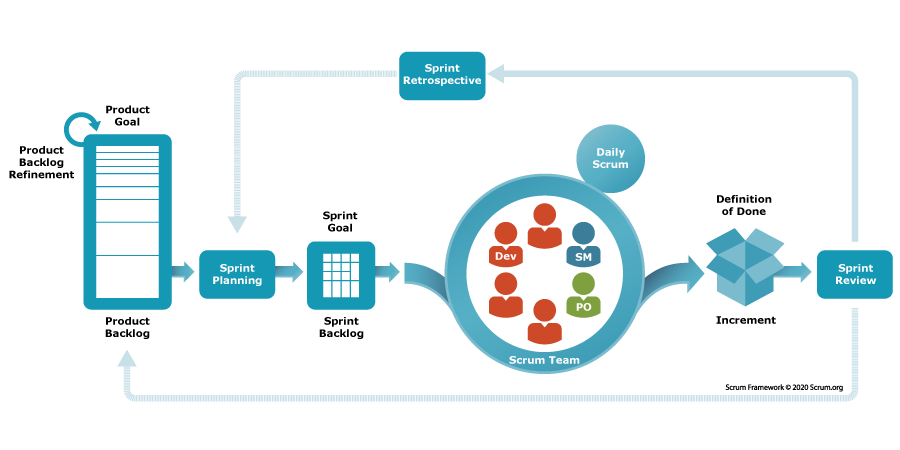
\includegraphics[width=0.6\linewidth]{Images//images/scrum.png}
    \caption{Life-cycle of the Scrum method}
    \label{fig:Life-cycle of the Scrum method}
\end{figure}

SCRUM is a framework for agile development. It is designed to add energy, focus, clarity, and transparency to project planning and implementation. At its core, SCRUM is about empowering a self-managing team to deliver, and it uses iterative, incremental practices to increase productivity and optimize predictability. In the context of our project, SCRUM provides a structured approach to managing the complex task of developing a new software product \cite{scrum}.

\subsection{SCRUM Roles}
Within the SCRUM framework, there are three key roles: the Product Owner, the Scrum Master, and the Development Team.

\vspace{10pt}

\begin{itemize}
\item \textbf{Product Owner:} The Product Owner is responsible for maximizing the value of the product resulting from the work of the Development Team. They manage the Product Backlog and are the sole person responsible for its content, availability, and ordering \cite{scrum}.

\item \textbf{Scrum Master:} The Scrum Master is responsible for promoting and supporting SCRUM. They do this by helping everyone understand SCRUM theory, practices, rules, and values. The Scrum Master serves the team by removing impediments to the team's progress \cite{scrum}.

\item \textbf{Development Team:} The Development Team is responsible for delivering potentially shippable increments of the product at the end of each Sprint. The team is self-organizing, cross-functional, and has all the skills necessary to create a product Increment \cite{scrum}.
\end{itemize}

\subsection{Product Backlog}
The Product Backlog is a list of features, functions, requirements, enhancements, and fixes that constitute the changes to be made to the product in future releases. It is the single source of requirements for any changes to be made to the product. The Product Owner is responsible for the Product Backlog, including its content, availability, and ordering \cite{scrum}.

\vspace{10pt}

\begin{itemize}
\item \textbf{Content:} The Product Backlog lists all features, functions, requirements, enhancements, and fixes that need to be made to the product. Each item in the backlog is expressed as a user story which provides a clear understanding of the requirement from an end-user perspective \cite{scrum}.
\item \textbf{Availability:} The Product Backlog is a living document that is available to all stakeholders. This ensures transparency and allows everyone involved in the project to understand the direction of the product and the work to be done \cite{scrum}.
\item \textbf{Ordering:} The items in the Product Backlog are ordered by the Product Owner based on their value, risk, priority, and necessity. This helps the Development Team to understand the work items' relative priority \cite{scrum}.
\end{itemize}

\subsection{The Sprint}
A Sprint is a time-boxed period during which specific work has to be completed and made ready for review. Sprints typically last between one week to one month. Here are the key aspects of a Sprint \cite{scrum}:

\vspace{10pt}

\begin{itemize}
\item \textbf{Sprint Planning:} At the start of the Sprint, the team holds a planning meeting to decide what work will be accomplished during the Sprint. The Product Owner identifies the items in the Product Backlog that he or she wants completed (the Sprint Goal) and the team decides how much of this they can commit to complete during the next Sprint \cite{scrum}.
\item \textbf{Daily Scrum:} Each day during the Sprint, the team holds a daily scrum meeting to discuss progress and plan for the day. This is not a problem-solving or issue resolution meeting. Instead, it is a chance for the team to inspect their progress towards the Sprint Goal and adjust their plan as necessary \cite{scrum}.
\item \textbf{Sprint Review:} At the end of the Sprint, the team holds a Sprint Review to inspect the Increment and adapt the Product Backlog if needed. During the Sprint Review, the Scrum Team and stakeholders collaborate about what was done in the Sprint \cite{scrum}.
\item \textbf{Sprint Retrospective:} After the Sprint Review and prior to the next Sprint Planning, the team holds a Sprint Retrospective. During this meeting, the team discusses what went well, what didn't, and how they can make improvements for the next Sprint \cite{scrum}.
\end{itemize}
